\chapter{Umsetzung}
\label{sec:Umsetzung}

\section{Motivation}

Dies Kapitel \dots

\chapter{Bewertung der Ergebnisse}
\label{sec:Bewertung}

\section{Motivation}

In Kapitel \ref{sec:Umsetzung} wurde der auf der Aufgabenstellung und den Erkenntnissen aus der Aufarbeitung zum Stand der Technik basierende Lösungsansatz und dessen Realisierung beschrieben. Bezogen auf unser Beispiel: Die Realisierung einer Web-Cam. 
Es sei angenommen, sie funktioniert. Nun stellt sich die Frage: Wie gut funktioniert sie? Wurden die in der Aufgabenstellung definierten Parameter durch die Realisierung erreicht? Wo liegen die Limitationen? Was funktioniert nicht? 
 
\section{Systemperformanz}
\label{sec:Performanz}
 
Dieses Kapitel gibt einen Einblick, unter welchen Parametern das Ergebnis getestet wurde und quantifiziert die Performanz des Systems. \\

\example Wie viele Bilder können von der Web-Cam pro Sekunde aufgenommen und verarbeitet werden? Gehen sporadisch Bilder verloren? Unter welchen Umgebungslichtbedingungen funktioniert die Schaferkennung - und unter welchen Bedingungen versagt diese? 

\begin{enumerate}
\item Testaufbau definieren
\item Messreihen durchführen
\item Messreihen analysieren
\end{enumerate}

Hierzu bietet sich die Darstellung der Ergebnisse durch eine Tabelle an, beispielhaft dargestellt durch Tabelle \ref{tab:Ergebnis}.

\begin{table}[htb]

\begin{tabular}{lcr}
  Spalte 1 & Spalte 2 & Spalte 3 \\
  1 & 2 & 3 \\
 \end{tabular}
 \caption{Testszenarios und Performanz}
\label{tab:Ergebnis}
\end{table}

Anhang/FAQ/häufige Fehler:

(Das Inhaltsverzeichnis ist nicht Bestandteil des Inhaltsverzeichnisses!)

Grobe Rechtschreibfehler sind durch Autokorrektur seltener geworden - jedoch im Bereich Zeichensetzung weisen Studierende große Wissenslücken auf. 
Wenn Sie Fragen zur Grammatik und Rechtschreibung haben, so sollten Sie nicht scheuen, den Blick in ein Fachbuch zu werfen. Es muss nicht immer der Duden sein, es existieren auch flüssig geschriebene, kompakte Nachschlagewerke auf den Markt. in ein kompaktes Buch nachzulesen - die investierte Zeit wird sich im Laufe Ihres Berufslebens schnell armortisieren!

Deutsche Grammatik und Rechtschreibung, Ines Balcik, Pons 2013

Ebenso verhält es sich mit mathematischen Definitionen, die Klarheit schaffen können. Auch hier gilt, bitte frischen Sie zur Projekt- oder Abschlussarbeit ihr Wissen im Bereich auf:

Mathematik für Informatiker, Band 1, Gerald Teschel, Susanne Teschl

Bei der Beurteilung von Messergebnissen: Bitte frischen Sie auch Ihr Wissen im Bereich Statistik auf, bzw. wählen Sie geeignete Informationen, um aus den daten Rückschlüsse zu ziehen. Hierzu gehört beispielsweise ein Histogramm, um die Verteilung der Messwerte darzustellen: Ist eine Normalverteilung gegeben? Was ist das nochmal? Dann zum Mittelwert auch die Frage beantworten: Wie stark streuen die Werte (Varianz)? Liegt keine Normalverteilung vor, dann ist Mittelwert + Varianz nicht das geeignete Mittel, Messwerte zu beurteilen. Beispiel: Grafik einer bimodalen Verteilung.

\begin{figure}
\begin{subfigure}[c]{0.5\textwidth}
	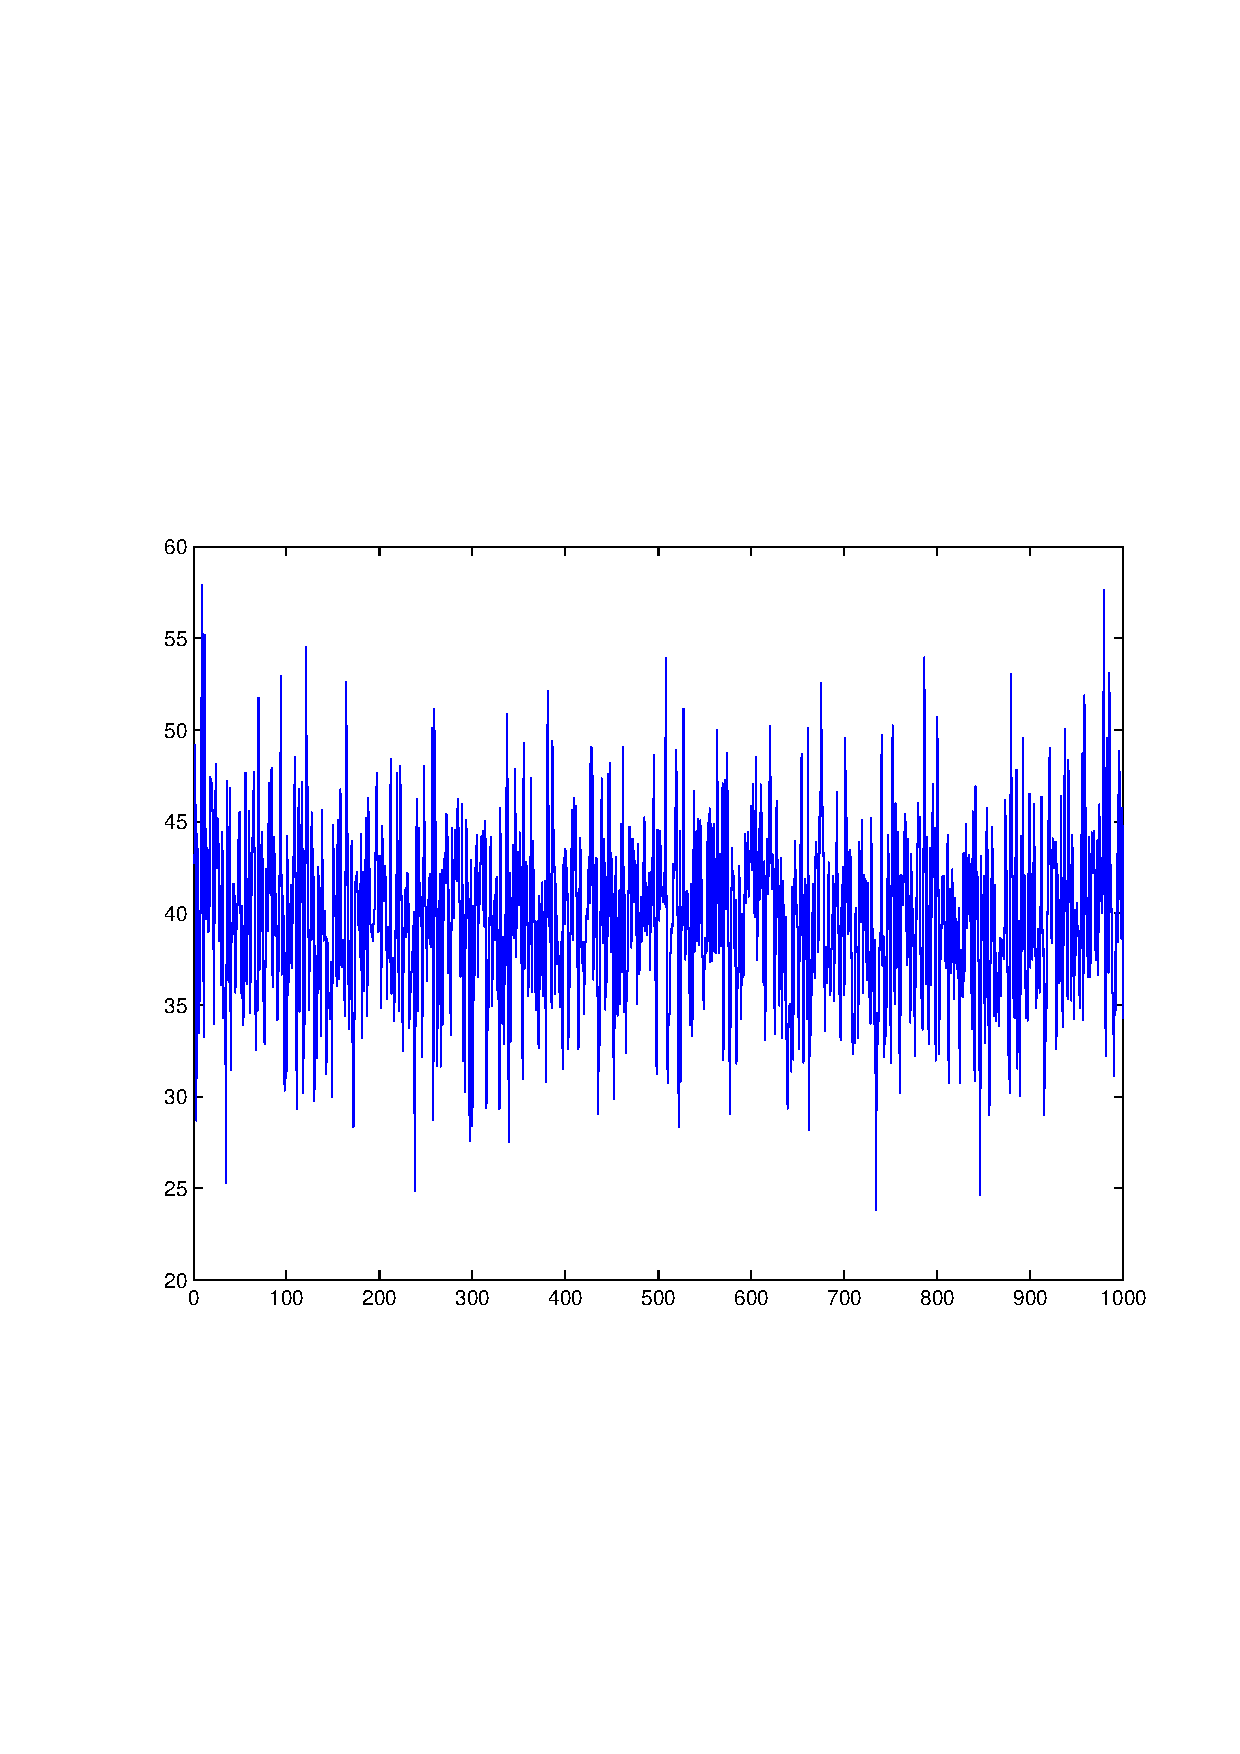
\includegraphics[trim = 25mm 75mm 15mm 90mm, clip, width=\textwidth]{matlab/statfig_10}
	\subcaption{Generierte Beispieldaten mit $\mu=40$ und $\sigma=5$}
\end{subfigure}
\begin{subfigure}[c]{0.5\textwidth}
	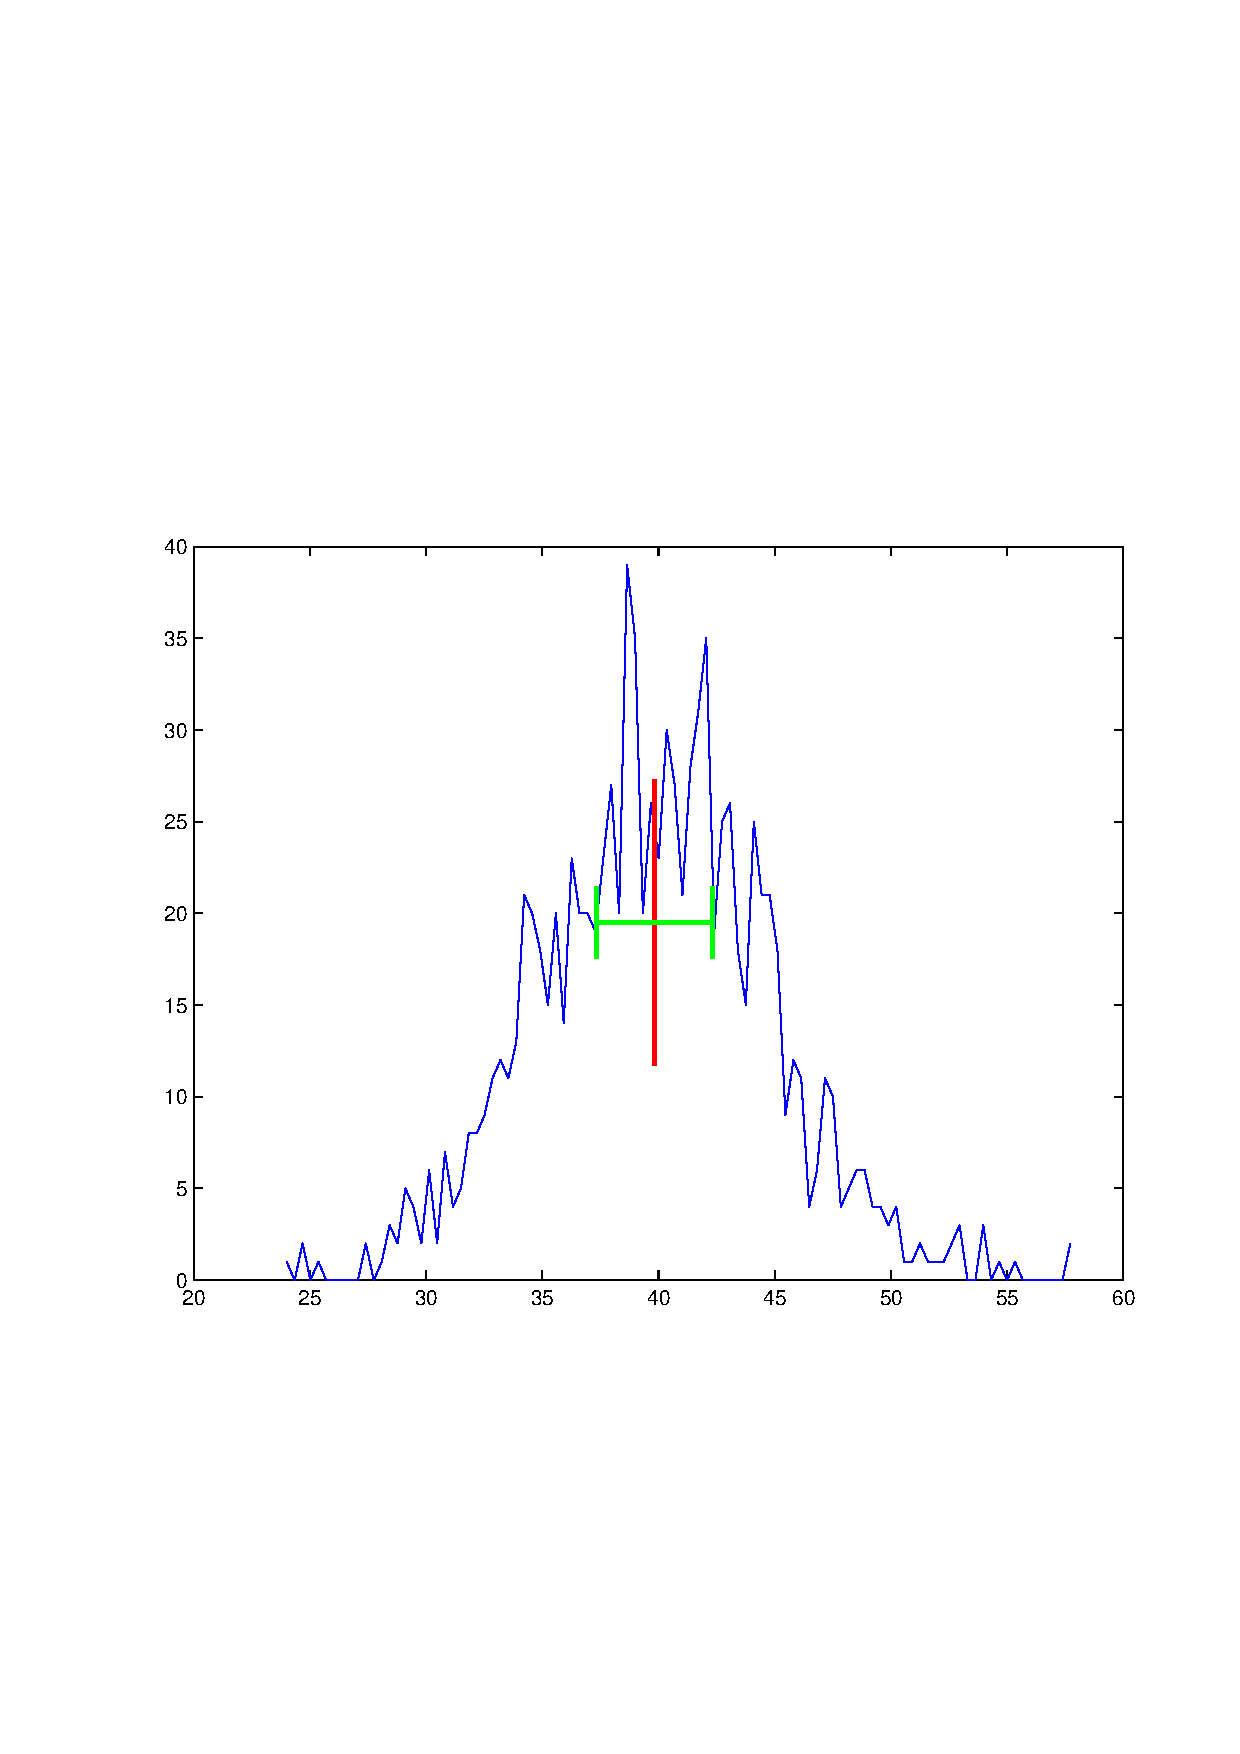
\includegraphics[trim = 25mm 75mm 15mm 90mm, clip, width=\textwidth]{matlab/statfig_20}
	\subcaption{Histrogramm der Beispieldaten aus (a).}
\end{subfigure}
\begin{subfigure}[c]{0.5\textwidth}
	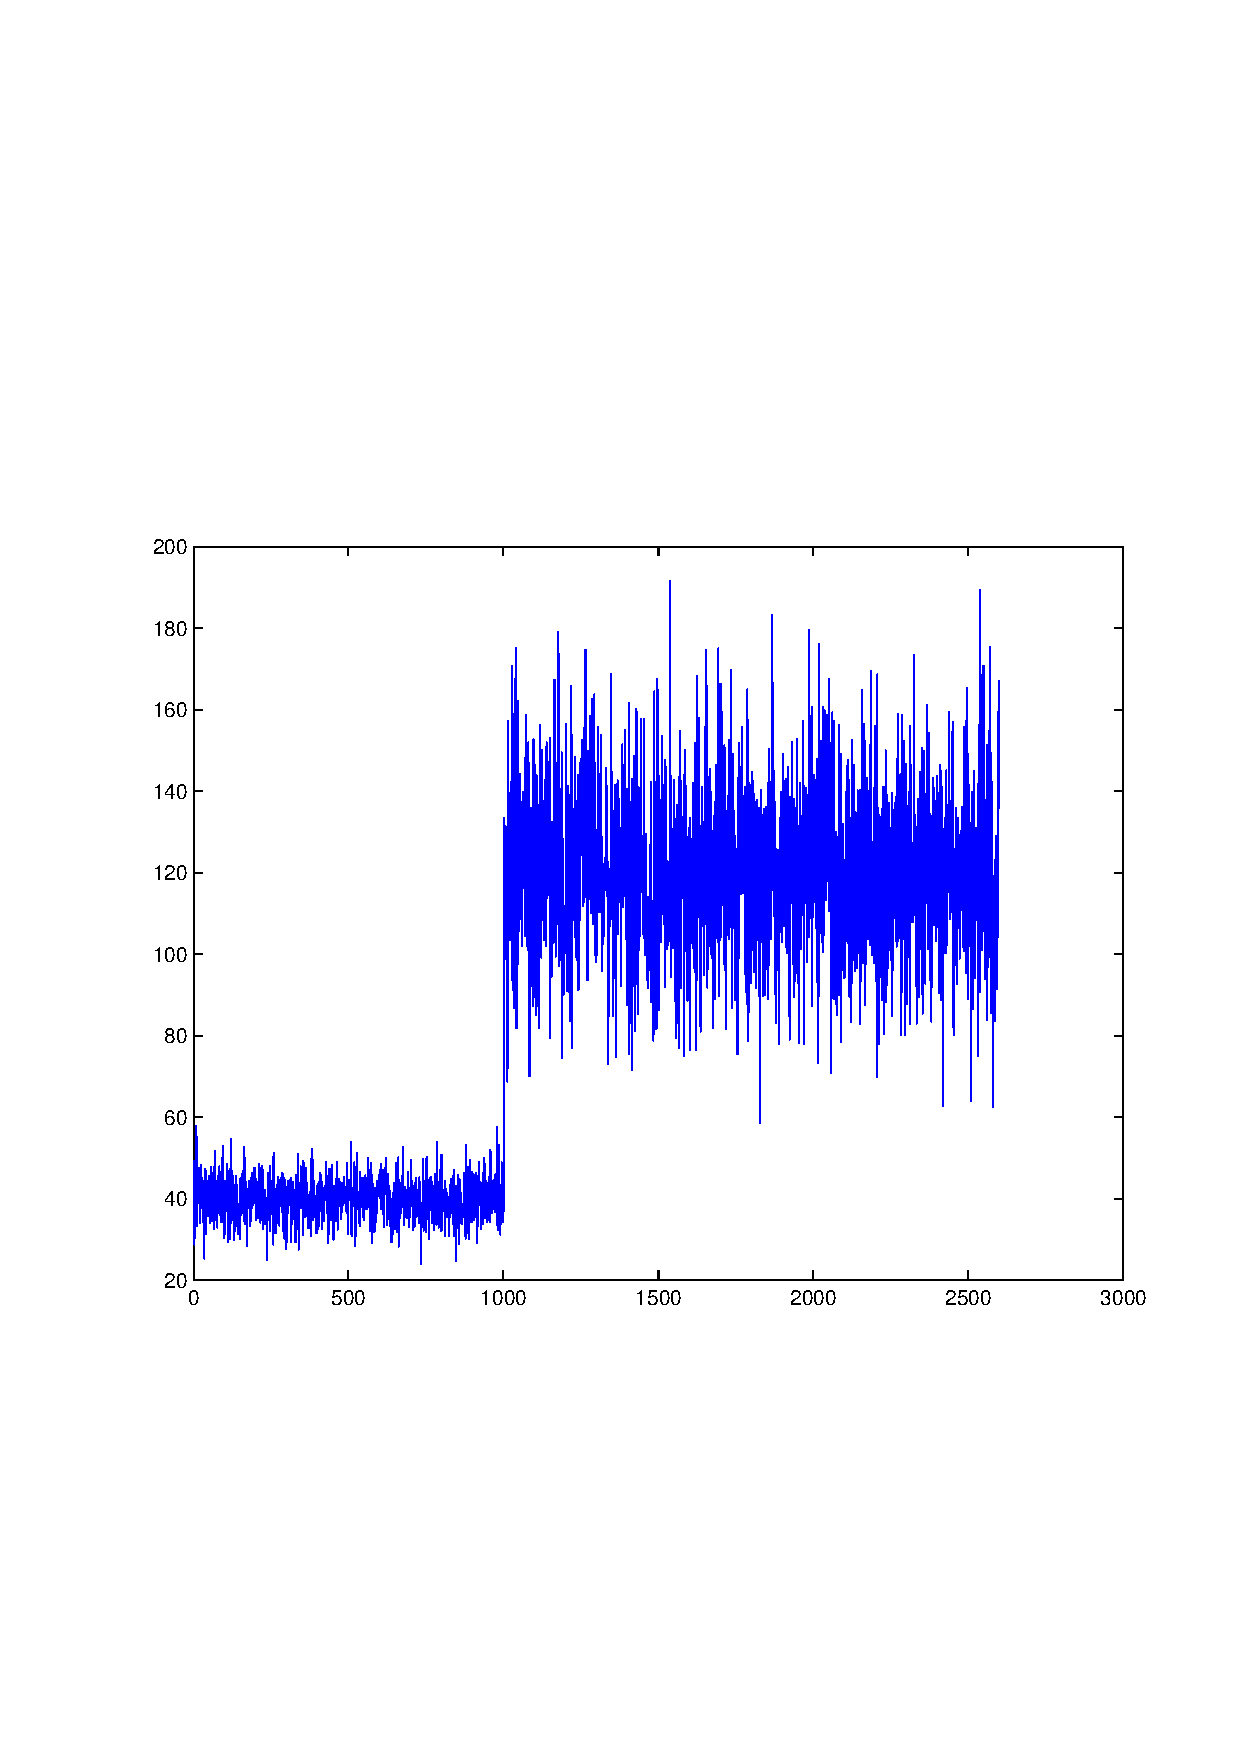
\includegraphics[trim = 25mm 75mm 15mm 90mm, clip, width=\textwidth]{matlab/statfig_30}
	\subcaption{Beispieldaten aus (a), gefolgt von Datenreihe mit $\mu=120$ und $\sigma=20$}
\end{subfigure}
\begin{subfigure}[c]{0.5\textwidth}
	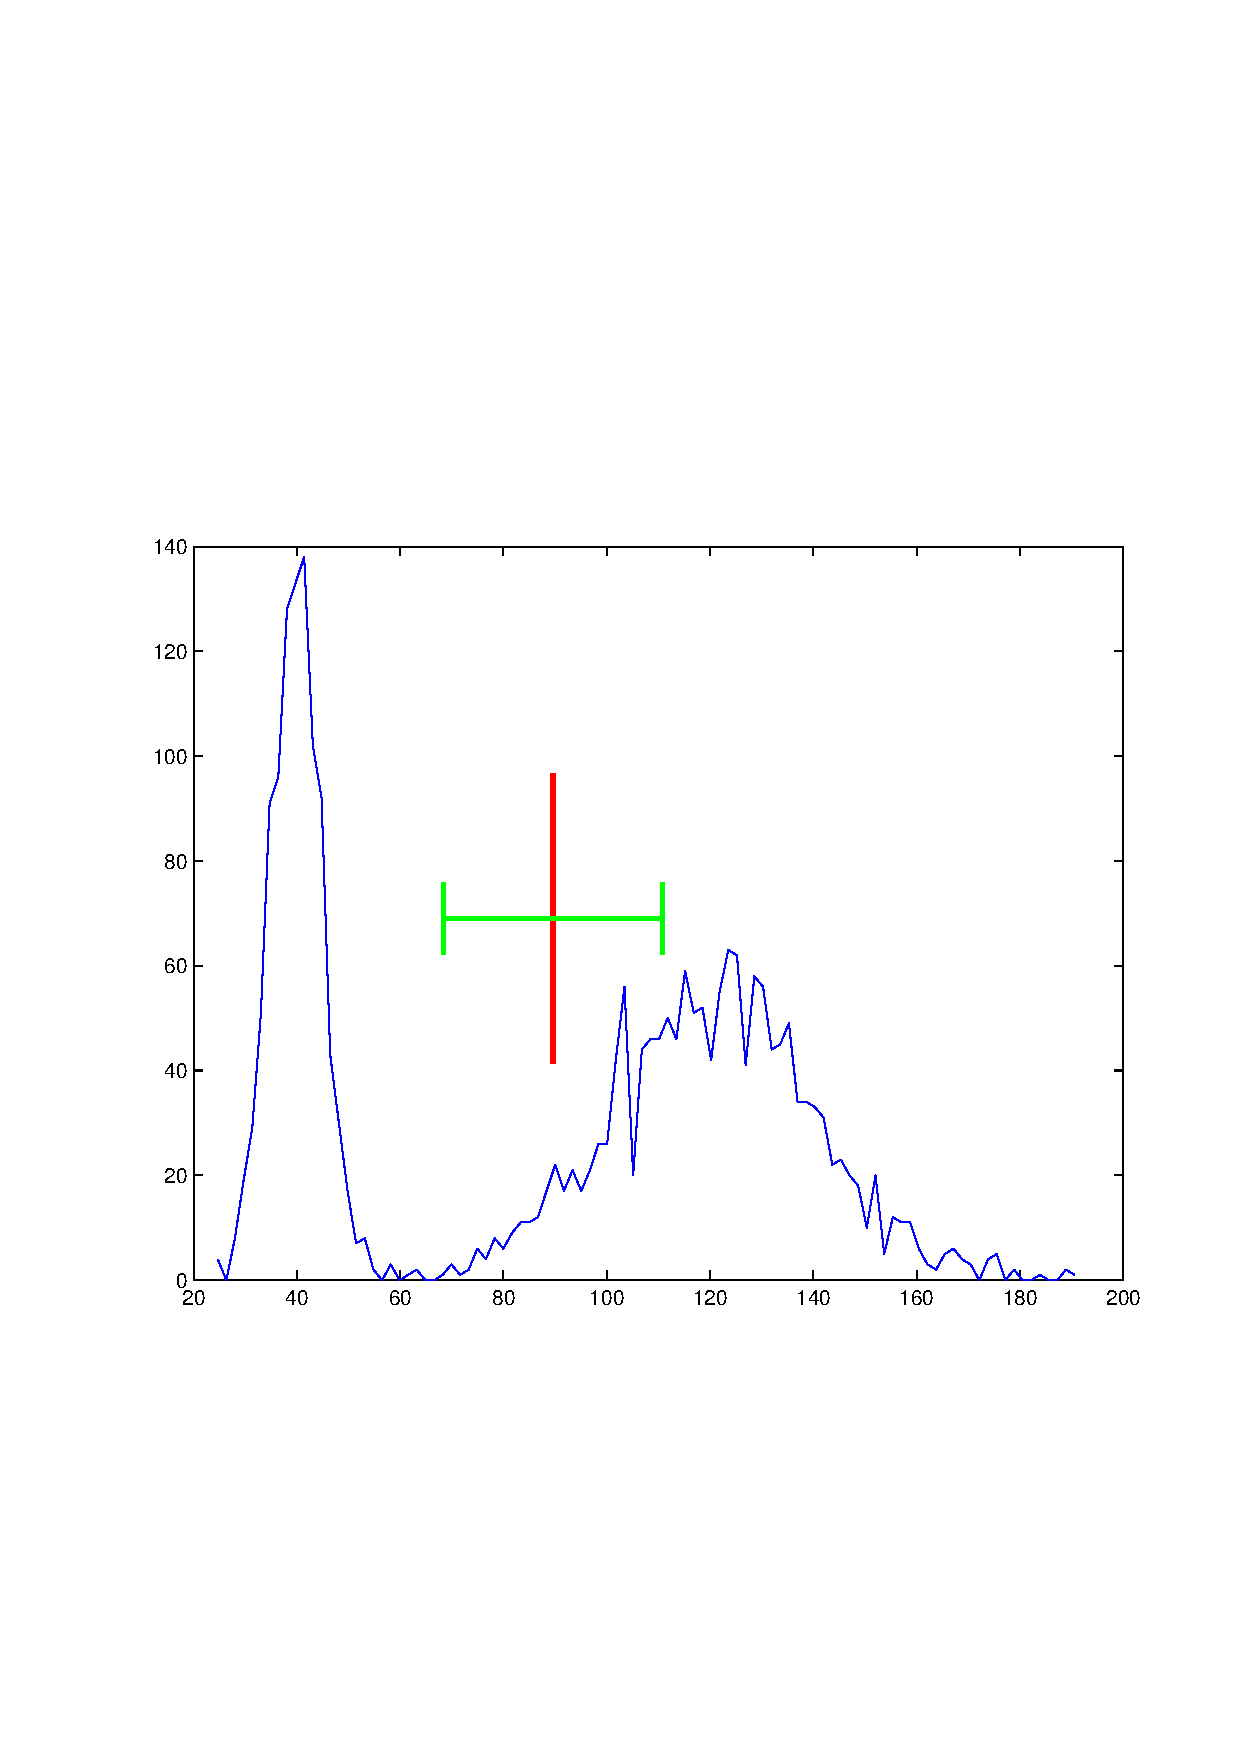
\includegraphics[trim = 25mm 75mm 15mm 90mm, clip, width=\textwidth]{matlab/statfig_40}
	\subcaption{Histrogramm der Beispieldaten aus (c).}
\end{subfigure}

\caption{Beispieldaten mit unimodaler und bimodaler Verteilung, siehe Listing \ref{lst:datagen}. Werden Messdaten visualisiert, bitte die Achsen mit entsprechenden Einheiten beschriften. \label{fig:Verteilung}}
\end{figure}

\begin{figure}
\begin{center}
	% zur Kontrolle der Abbildungsränder kann \fbox{} genutzt werden
	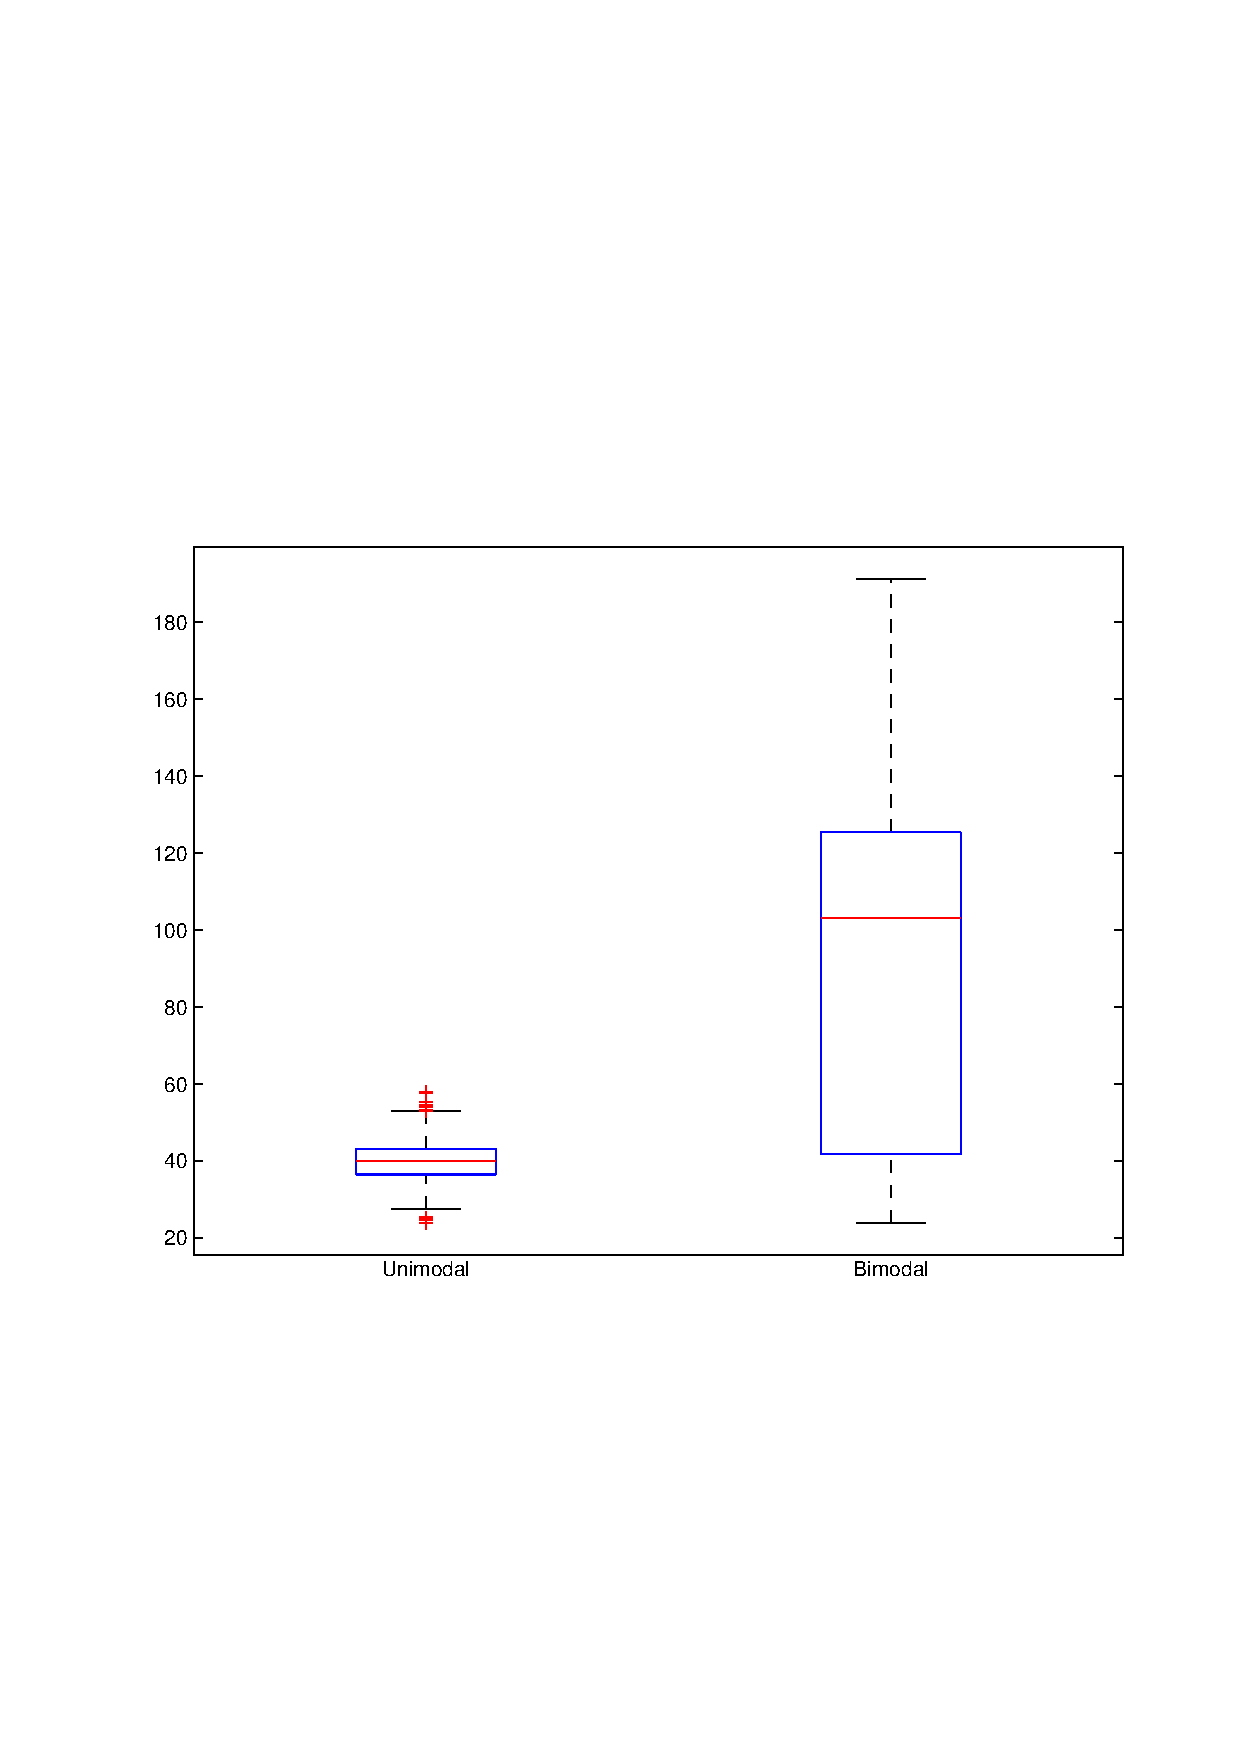
\includegraphics[trim = 25mm 75mm 15mm 90mm, clip, width=8cm]{matlab/statfig_50}
\caption{''Boxplot'' zur Visualisierung der Verteilung von Beispieldaten aus Abbildung \ref{fig:Verteilung}.\label{fig:Boxplot}}
\end{center}
\end{figure}

Weitere ToDo

+ latex-Style-File überarbeiten/aufräumen: nicht zwingend notwendige Pakete/Extras in das Hauptdokument überführen

+Erklärung(en) überarbeiten/aktualisieren  
